\subsection{\label{sec:processLayout}Layout of a Process Environment}
As mentioned above, the top-level element of a \streams process
definition is a {\em container}. A single container may contain
multiple processes, streams and services, which are all executed in
parallel. An example for a container definition is provided in
Figure \ref{fig:simpleContainer}.

\begin{figure}[h!]
	\begin{lstlisting}[showstringspaces=false]
      <container id="example">
          <stream id="D" url="file:/test-data.csv" />

          <process input="D">
               <!--
                   The following 'PrintData' is a simple processor that outputs each
                   item to the standard output (console)
                 -->
               <stream.data.PrintData />
          </process>
      </container>
	\end{lstlisting}
	\caption{\label{fig:simpleContainer}A simple container, defining a stream that is created from a CSV file.}
\end{figure}

The core XML elements used in the simple example of Figure
\ref{fig:simpleContainer} are {\ttfamily stream} and {\ttfamily
  process}, which correspond to the conceptual elements that have
previously been introduced in Section \ref{sec:abstraction} and
which are mapped to XML elements according to Table \ref{tab:xmlElements}.
This example defines a container with namespace {\ttfamily example}
which corresponds to the simple compute graph shown in Figure
\ref{fig:simpleGraph}.

\begin{figure}[h!]
  \centering
  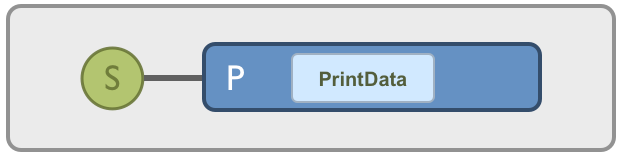
\includegraphics[scale=0.3]{graphics/simple-graph}
  \caption{\label{fig:simpleGraph}The simple compute graph that is
    defined by the XML given in Figure \ref{fig:simpleContainer}.}
\end{figure}

The graph contains a single source of data ({\em stream}) and only
one {\em process} element, which consumes the data provided by the
stream and applies the nested processor {\ttfamily PrintData} to
each data item obtained from the stream.

\subsubsection{\label{sec:defineStream}Defining a Stream Source}
As you can see in the example above, the {\ttfamily stream} element is used to define
a stream object that can further be processed by some processes. The {\ttfamily stream}
element requires an {\ttfamily id} to be specified for referencing that stream as input
for a process. 

In addition, the {\ttfamily url} attribute is used to specify the location
from which the data items should be read by the stream. There exists Java implementations
for a variety of data formats that can be read. Most implementations can also handle 
non-file protocols like {\ttfamily http}. The class to use is picked by the extension
of the URL ({\ttfamily .csv}) or by directly specifying the class name to use:
\begin{figure}[h!]{\footnotesize
    \centering
    \begin{lstlisting}{lang=xml}
       <stream  id="D" class="stream.io.CsvStream"
               url="http://download.jwall.org/stuff/test-data.csv" />
    \end{lstlisting}
    \caption{\label{fig:defStream}Defining a stream that reads from a HTTP resource.}
}
\end{figure}

Additional stream implementations for Arff files, JSON-formatted files or for reading 
from SQL databases are also part of the {\em streams} library. These implementation
also differ in the number of parameters required (e.g. the database driver for SQL
streams). A list of available stream implementations can be found in Appendix \ref{api:stream:io}.
The default stream implementations also allow for the use of a {\ttfamily limit} parameter
for stopping the stream after a given amount of data items.

\subsubsection{A Stream Process}
The {\ttfamily process} element of an XML definition is associated
with a data stream by its {\ttfamily input} attribute. This references
the stream defined with the corresponding {\ttfamily id}
value. Processes may contain one or more {\em processors}, which are
simple functions applied to each data item as conceptually shown in
\ref{sec:basics}.

A process will be started as a separate thread of work and will read
data items from the associated stream one-by-one until no more data
items can be read (i.e.  {\ttfamily null} is returned by the
stream). Processes in the \streams framework are following greedy
strategy, reading and processing items as fast as possible.

The processes will apply each of the nested processors to the data
items that have been read from the input. The processors will return
a processed data item as result, which is in turn the input for the
next processor embedded into the process. Thus, each process applies
a pipeline of processors to each data item. If any processor of the
pipeline returns {\ttfamily null}, i.e. no resulting data item, then
the pipeline is stopped and the process skips to reading the next
data item from the stream.

The inner processors of a process are generally provided by Java
implementations and are represented by XML elements that reflect
their Java class name. 

In the example in Figure \ref{fig:processXml}, a processor implemented
by the class {\ttfamily my.package.MyProcessor} is added to the
process. The process in this examples is attached to the stream or
queue defined with ID {\ttfamily id-of-input}. Any output of that
process that is not {\ttfamily null}, will be inserted into the queue
with ID {\ttfamily queue-id}. Connecting the output of a process to a
queue (which can then be the input to another processor) is optional.

\begin{figure}[h!]
  \centering
  \begin{lstlisting}
    <process input="id-of-input" output="queue-id">
        <!-- 
             One or more processor elements, referenced
             by their class name, provided with attributes
           -->
        <my.package.MyProcessor param="value" />
    </process>
  \end{lstlisting}
  \caption{\label{fig:processXml}A process references an input
    (i.e. a {\em stream} or a {\em queue}) and contains a list of
    processor elements. Optionally it feeds results to an associated
    output (a {\em queue}).}
\end{figure}

%The general behavior of a process is shown in the pseudo-code
%of Algorithm \ref{alg:process}.
%
%\begin{algorithm}
%\begin{algorithmic}
%\Require{ A data stream $S$ and a sequence $P = \langle f_1,\ldots,f_k\rangle$ of processors}
%\Statex
%\Function{ProcessStream}{$S$}
%   \While{ $true$ }
%      \State{$d :=  \textrm{readNext}( S )$}
%      \ForAll{ $f \in P$ }
%         \State{$d' := f(d)$}
%         \If{$d' = null$}
%         	\Return{$null$}
%         \Else
%	         \State{$d := d'$}
%         \EndIf
%      \EndFor
%   \EndWhile
%\EndFunction
%\end{algorithmic}
%\caption{\label{alg:process}Pseudo-code for the behavior of a simple {\ttfamily process} element.}
%\end{algorithm}

\subsubsection{Processing Data Items}
As mentioned in the previous Section, the elements of a stream are
represented by simple tuples, which are backed by a plain hashmap of
keys to values. These items are the smallest units of data within the
\streams library. 

The smallest {\em functional} units of the \streams library are
provided by simple {\em processor}s.  A {\em processor} is essentially
a function that is applied to a data item and which returns a data
item (or {\ttfamily null}) as result as shown in the {\em identity}
function example below.
\begin{figure}[h!]
   \begin{lstlisting}[language=Java,showstringspaces=false]
	    public Data process( Data item ){
	    	return item;
	    }
   \end{lstlisting}
   \caption{\label{fig:processMethod}The {\ttfamily process(Data)} method - unit of work within {\em streams}.}
\end{figure}

Processors are usually implemented as Java classes, but can be
provided in other (scripting) languages as well. The Java classes are
expected to follow the JavaBeans specification by providing {\ttfamily
  get}- and {\ttfamily set}-methods for properties.  These properties
in turn will be mapped to XML attributes of the corresponding XML
element. This allows processors to be easily provided with parameters
wihtin the XML container definitions.
